%%%%%%%%%%%%%%%%%%%%%%%%%%%%%%%%%%%%

Figure~\ref{fig:truth:dphipt} shows the gluon jet $p_\text{T}$ dependence of the $\Delta\phi$ observable.  Interestingly, Pythia predicts that the difference between polarization on and off should grow with $p_\text{T}$.  Similarly, Fig.~\ref{fig:truth:dphi2} shows that they increase also with mass (and the correlated $\Delta R$ and $z$).  This would be an interesting feature to try to expose with future measurements.

\begin{figure}[htbp]
  \centering
 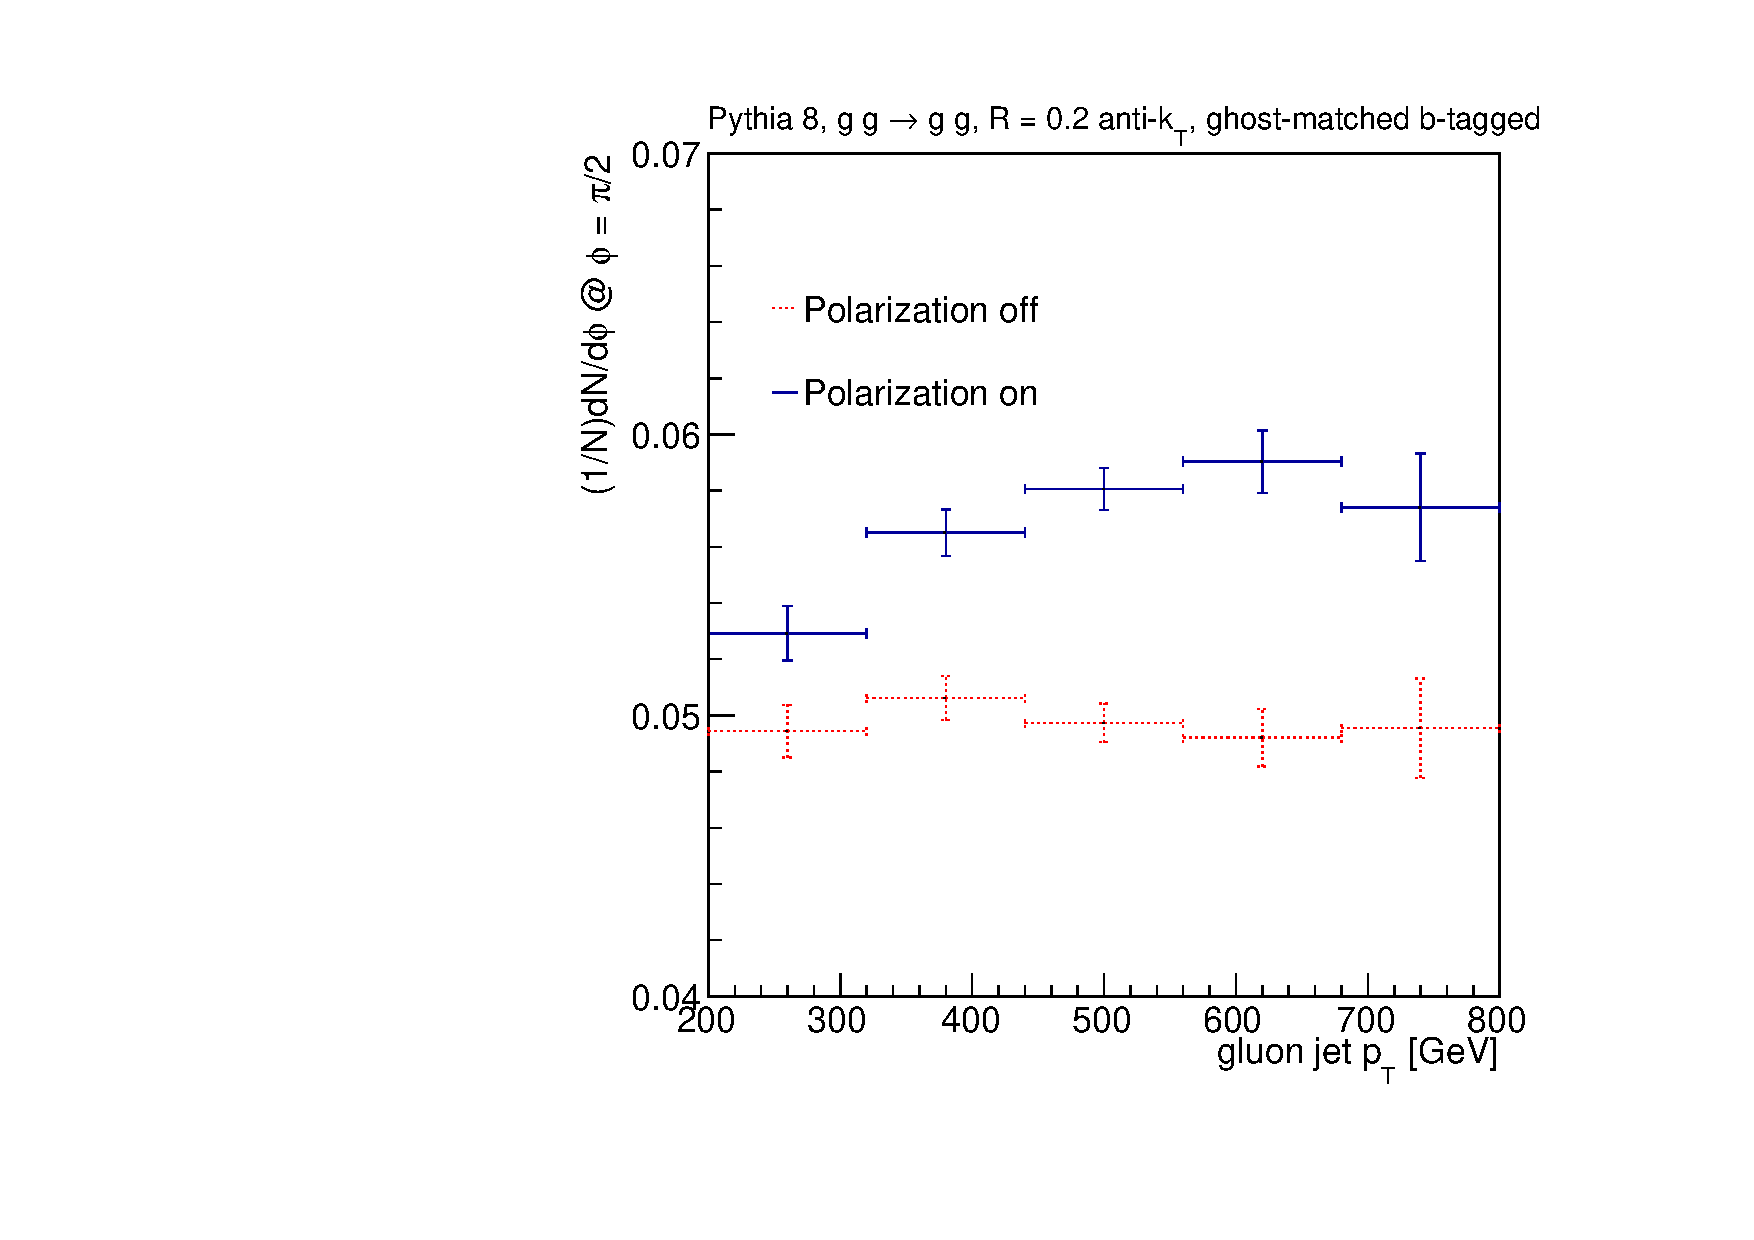
\includegraphics[width=0.5\textwidth]{figures/truth_level/dphi_versus_pt}

\caption{The dependence of the value of the normalized histogram of the $\Delta\phi$ variable as a function of the gluon jet $p_\text{T}$. }
  \label{fig:truth:dphipt}
\end{figure}


\begin{figure}[htbp]
  \centering
 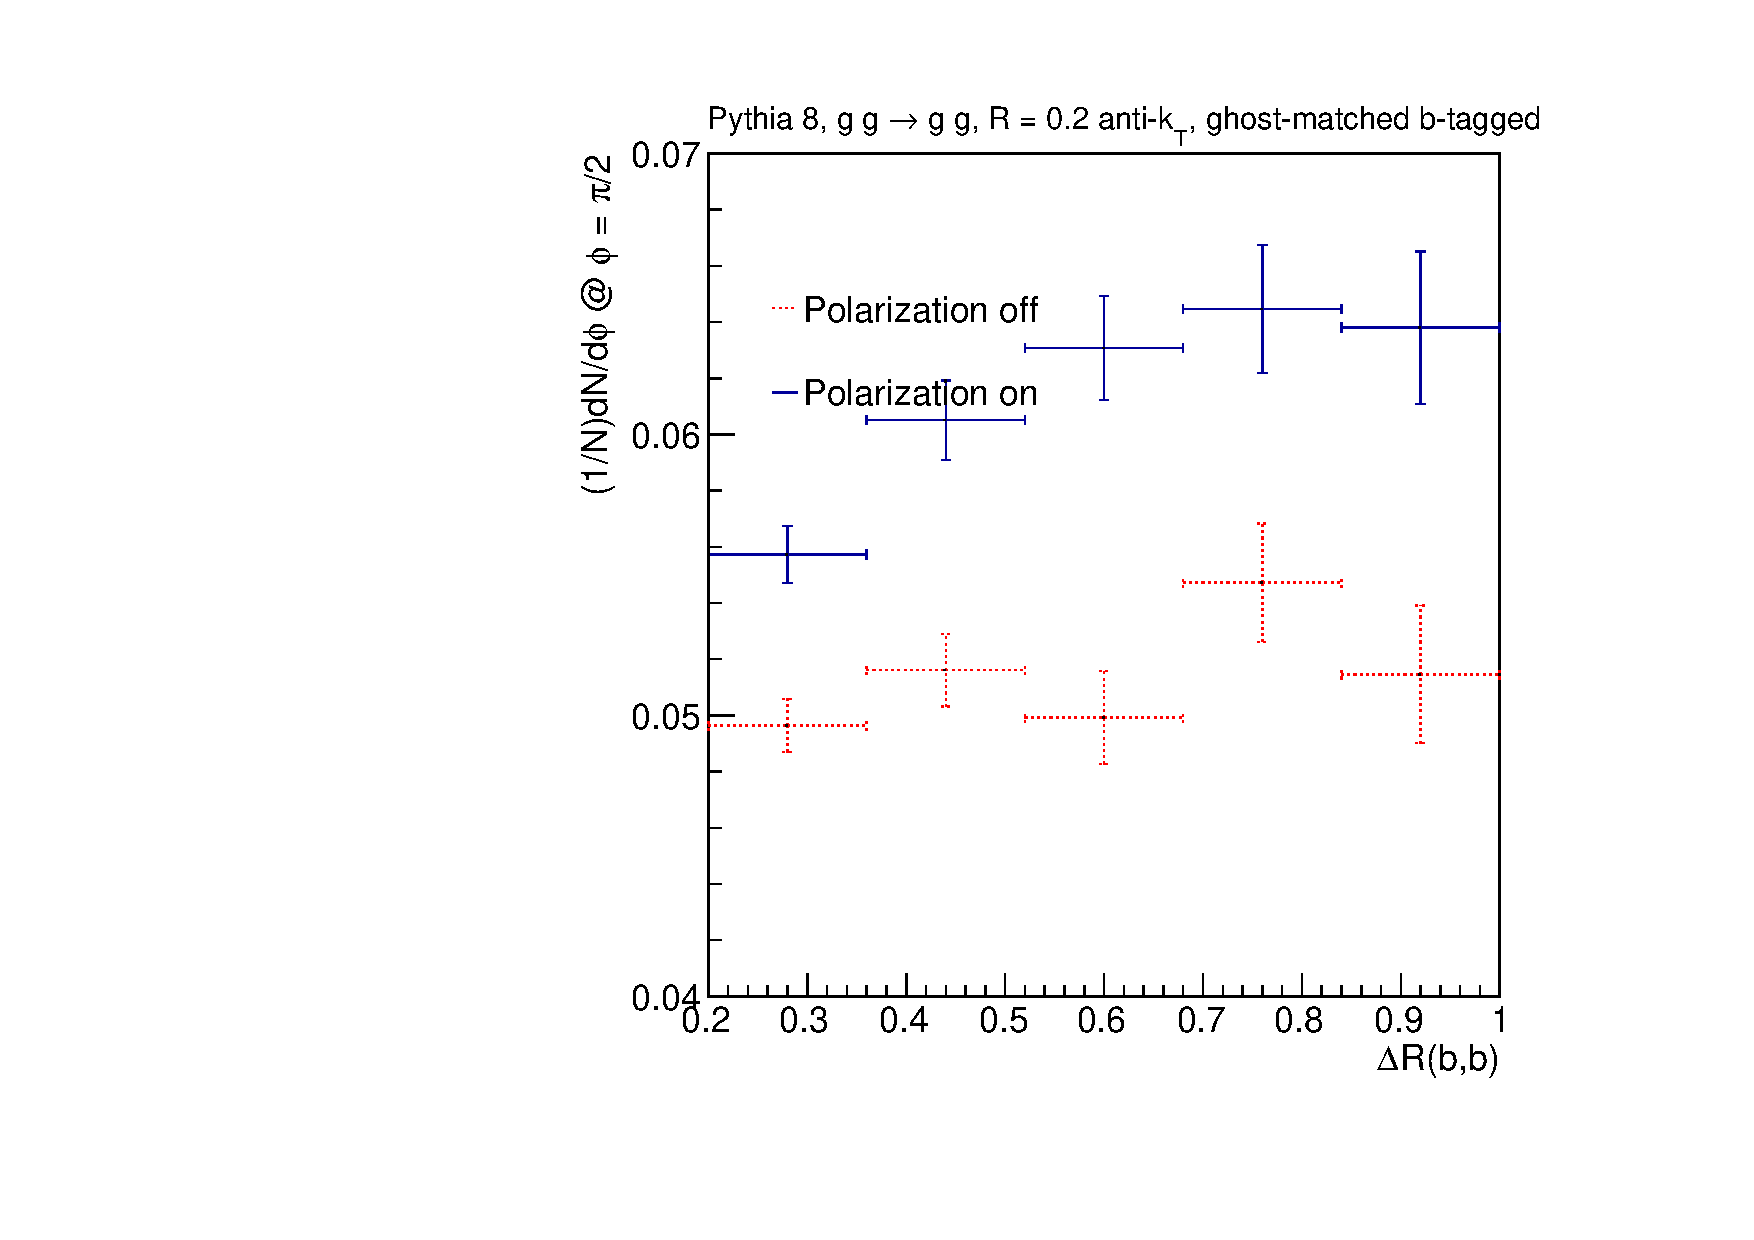
\includegraphics[width=0.5\textwidth]{figures/truth_level/dphi_versus_dR.pdf}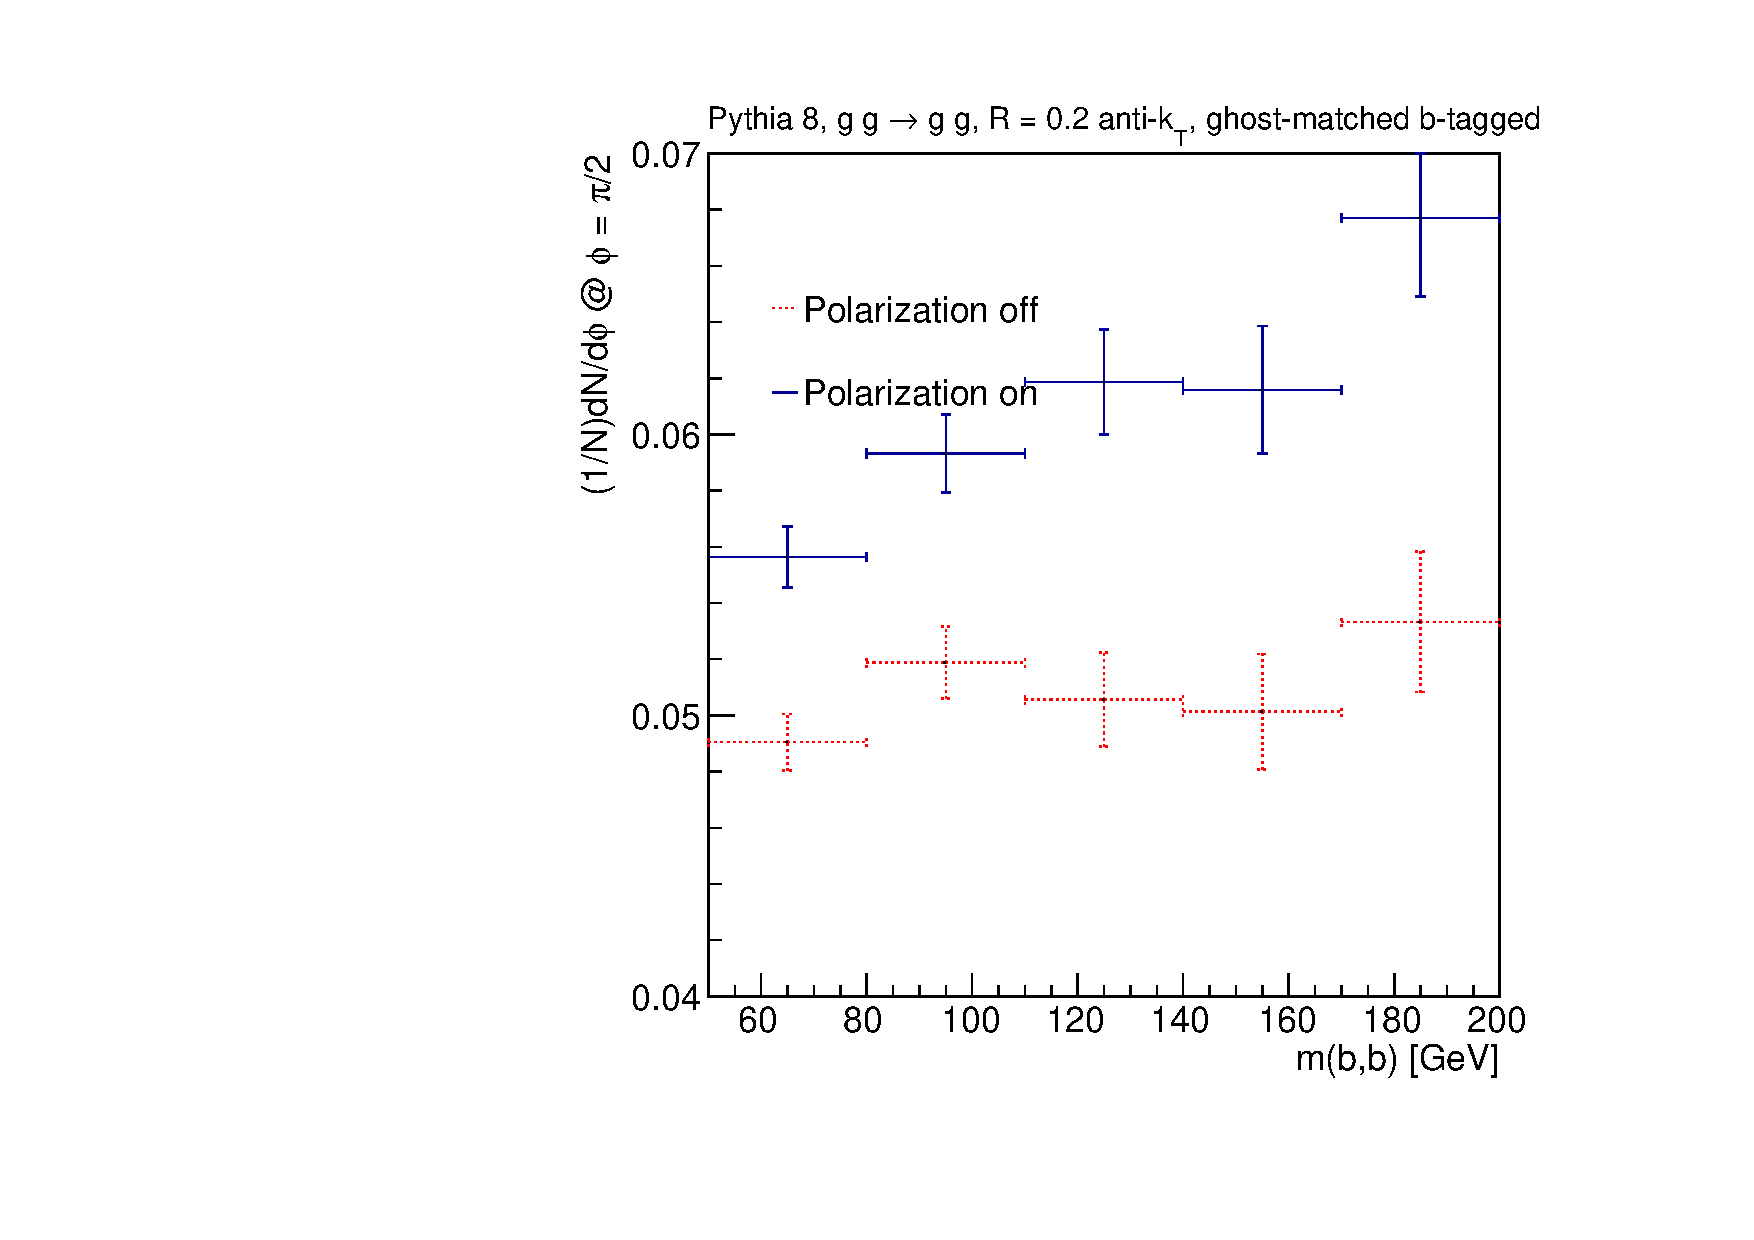
\includegraphics[width=0.5\textwidth]{figures/truth_level/dphi_versus_m.pdf}\\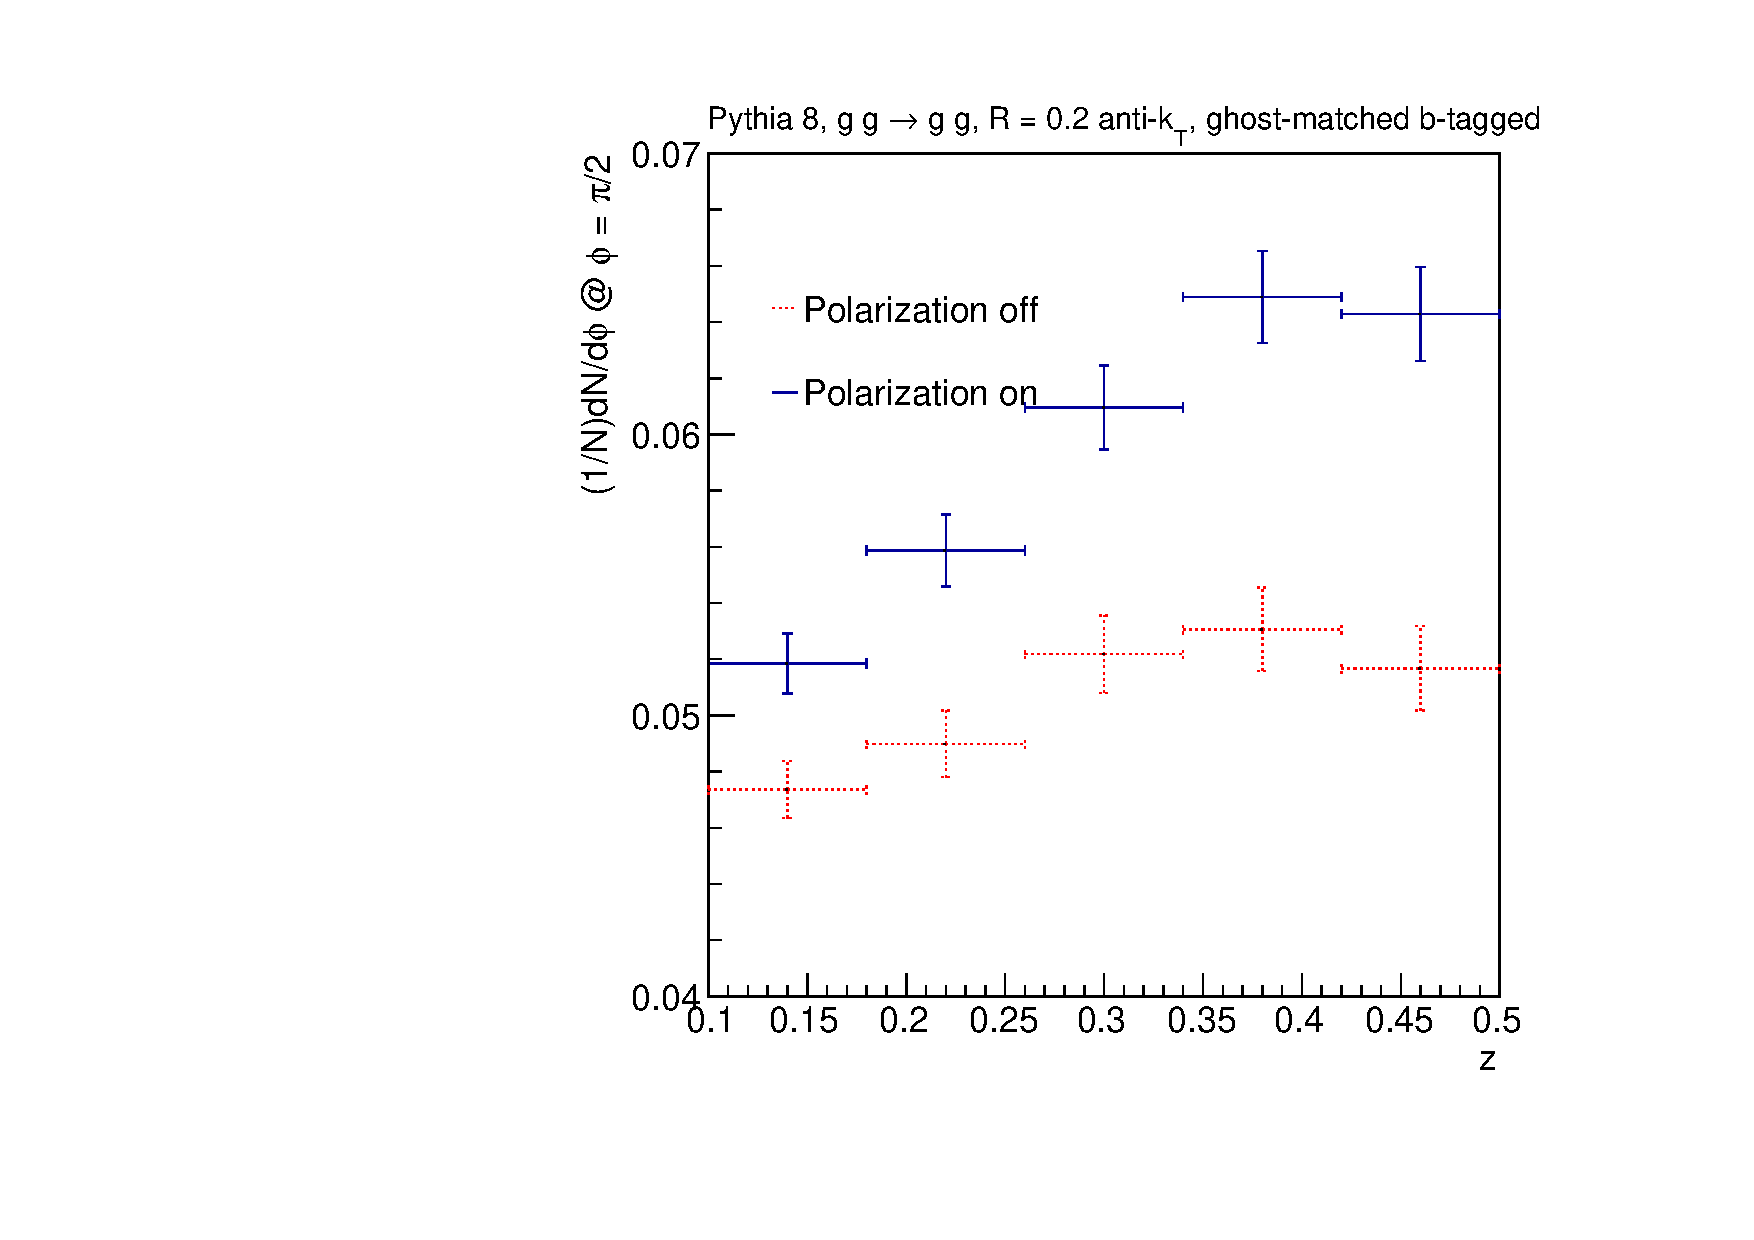
\includegraphics[width=0.5\textwidth]{figures/truth_level/dphi_versus_z.pdf}

\caption{The dependence of the value of the normalized histogram of the $\Delta\phi$ variable as a function of $\Delta R$, $m(b,b)$ and $z(b,b)$. }
  \label{fig:truth:dphi2}
\end{figure}



